\documentclass{article}

\usepackage[english]{babel}
\usepackage[a4paper]{geometry}
\usepackage{amsmath}
\usepackage{graphicx}
\usepackage[colorlinks=true, allcolors=blue]{hyperref}
\usepackage{pgf}
\usepackage{xcolor}

\title{Project Plan - Agents with Small Language Models}
\author{Paulo Ricardo Beckhauser de Araujo - s242779}

\begin{document}
\maketitle

\section*{Motivation}
% Present the context and significance of the problem you aim to address.
% Explain why this topic matters within your field and what gap it fills.
% Discuss relevant prior work and how your project builds on it.
% This section should be approximately half to one page in length.
% Use this space to clarify the problem’s importance and real-world relevance.

Recent progress in agentic systems has primarily resulted from the
development of increasingly large language models \cite{Andreas2022Language}, whose scale facilitates
intricate reasoning, tool usage, and structured interactions.
However, reliance on large models poses major challenges, including elevated
computing costs, elevated latency, greater deployment complexity, and
restricted accessibility in resource-constrained settings.
This situation motivates an investigation into whether current agent
capabilities are inherently tied to model scale, or whether comparable
reliability and functionality can be achieved through enhanced system design
using smaller language models \cite{Zhang2025The} and \cite{Belcák2025Small}.

This thesis is motivated by the hypothesis that many shortcomings observed in
agentic systems, including unreliable function calls, malformed structured
outputs, and nondeterministic behavior, emerge primarily from insufficient
constraints during generation rather than from model size.
Constrained decoding and structural enforcement techniques deliver an
effective alternative, enabling smaller language models to generate outputs
that strictly adhere to fixed schemas and execution plans \cite{Beurer-Kellner2024Guiding}.
Guiding generation through formal constraints may enable predictable,
production-ready agent behavior without reliance on ever-larger models.

This research aims to determine whether techniques currently employed in
large-model agentic systems can be effectively replicated using small
language models when supported by constrained decoding.
Demonstrating this capability would help decouple agent reliability from
model scale, thereby enabling the development of lightweight, cost-efficient,
and locally deployable agents suitable for enterprise, embedded, and
privacy-sensitive applications.

Ultimately, this research seeks to contribute to a shift in focus from
scaling models to improving system-level reliability, demonstrating that
dependable agentic systems can be built through structural and algorithmic
improvements rather than computational scale alone.

\section*{Background}

One of the main challenges for LLM-based agents is reliably generating
structured outputs, especially when calling functions or tools. These models
need to follow specific schemas, using valid function names and correct
argument types. However, when generation is not controlled, outputs can be
malformed, may contain missing fields, or may include tools that do not exist.
This often means more post-processing and repeated queries, which makes the
system less efficient and reliable.

To solve these problems, some research has explored constrained decoding \cite{Geng2023Grammar-Constrained} and
structural enforcement. This makes language generation a controlled process,
improving consistency and accuracy in agent workflows. For function and tool
calls, constrained decoding lets models choose only from registered functions
and create arguments that meet the required specifications, helping avoid
common errors in small and medium-sized models.

Also, several methods have been developed to make small language models more
efficient, including knowledge distillation \cite{Hinton2015Distilling}, low-rank factorization \cite{hu2021loralowrankadaptationlarge},
quantization \cite{Liang2021Pruning}, and pruning \cite{Han2015Deep}. These techniques reduce the need for computing power
and memory, enabling the models to run on devices with limited resources.
However, these methods do not directly improve output reliability, and smaller
or compressed models can still produce invalid outputs if decoding is not
controlled. Methods and decoding-level control are largely complementary.
Integrating lightweight models with structural enforcement mechanisms provides
a pathway to systems that are both computationally efficient and behaviorally
reliable. 

In this context, the thesis points to constrained decoding for function and
tool calling as a key way to achieve reliable behavior in small language
models. By studying structural enforcement alongside efficiency methods, this
research examines how careful system design can compensate for limited model
capacity and help build controllable, efficient agent systems.

\section*{Research Question}
% Formulate a clear and focused research question that guides your project.
% The question should be specific, answerable, and grounded in the scientific method \cite{scientific_method}.
% Briefly describe the hypothesis or assumptions underlying your investigation.
% Explain how answering this question will contribute new knowledge or insight.

Can reliable agentic behavior, particularly in function calling and structured
output generation, be achieved using small language models when constrained
decoding techniques are applied, thereby reducing dependence on large-scale
models for production-grade agent systems?

This research is based on the assumption that many reliability issues in
current agentic systems arise not only from limited model capability but also
from unconstrained generation processes that permit outputs to deviate from
expected structures.
The central hypothesis is that enforcing structural constraints during
decoding enables small language models to achieve levels of correctness,
determinism, and robustness comparable to those of larger models in agent
scenarios requiring precise tool invocation and structured responses.

Addressing this question provides new insight into whether advances in
agentic AI primarily depend on model scale or on improvements in generation
control and system design.
Demonstrating that constrained decoding can enable dependable agent behavior
in small models would support the development of more efficient,
cost-effective, and deployable AI systems, particularly in environments with
limited computational resources or where local deployment is necessary.

\section*{Time plan}
% Present a time plan in the form of a Gantt chart outlining your project
% phases.
% Include milestones such as literature review, implementation, testing, and
% writing.
% Add a short risk analysis discussing possible delays in different phases.
% For each risk, briefly describe mitigation strategies or contingency plans.
% Ensure your plan is realistic and aligns with your available time and
% resources.

% \section*{References}
The main phases of this thesis are outlined below. An overview of the
timetable associated with these phases is provided in Fig.~\ref{fig:timetable}.


\begin{figure}[ht]
\centering
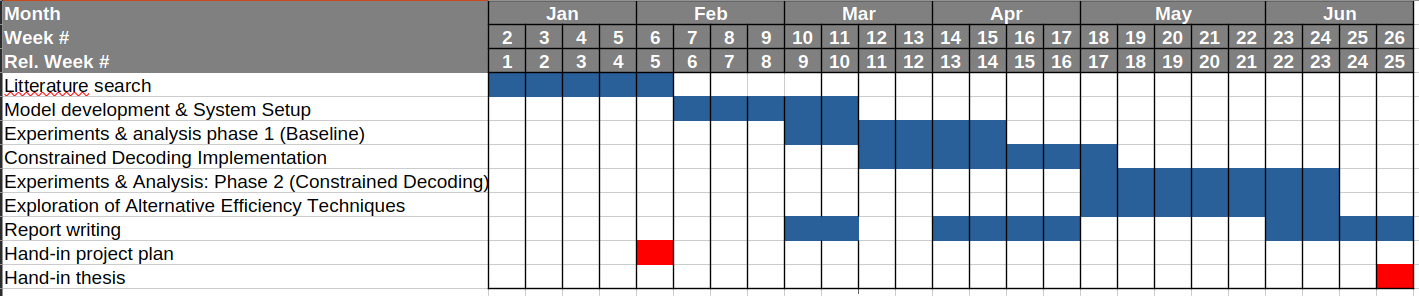
\includegraphics[width=0.8\textwidth]{time_plan.png}
\caption{Gantt chart of the project plan.}
\label{fig:timetable}
\end{figure}

Several risks may impact the project timeline. The literature review phase could
extend beyond initial estimates if relevant prior work is broader or more
fragmented than anticipated, potentially delaying subsequent design decisions.
Model development and system setup may encounter technical challenges related
to framework compatibility, hardware limitations, or unforeseen implementation
complexity.

During the experimental phases, delays may arise from unstable model behavior,
longer-than-expected training or inference times, or the need to repeat
experiments to ensure statistical validity. Exploring alternative efficiency
techniques, such as knowledge distillation or model compression, carries the
risk of limited performance gains or increased engineering overhead, which may
reduce the depth of analysis achievable within the allocated timeframe. To
mitigate these risks, the project prioritizes constrained decoding as the core
contribution and maintains flexibility in the scope of complementary techniques.

Finally, report writing may be affected by delays in earlier phases. To address
this, writing is scheduled to overlap with experimentation to ensure steady
progress toward the final submission.

\newpage

\nocite{*}
\bibliographystyle{unsrt}
\bibliography{bibliography}

\end{document}
